\documentclass[10pt,a4paper]{article}
\usepackage[english]{babel}
\usepackage[utf8]{inputenc}
\usepackage{fullpage}
\usepackage{textcomp}
\usepackage{graphicx}
\usepackage{hyperref}
\usepackage{url}
\usepackage{caption}
\usepackage{float}
\usepackage{minted}
\usepackage{datetime}

\usepackage{subfigure}
\urlstyle{same}

\begin{document}

\begin{titlepage}
\begin{center}
\textsc{\huge \bfseries Advanced Networking 2018}\\[1.5cm]
\textsc{\large Lab \#3: Build a Net}\\[1.5cm]
\textsc{\huge Report}\\[1.5cm]
\textsc{\huge \bfseries GROUP: 3}\\[1.5cm]
\textsc{\large{\textbf{Authors:}\\ 
Kotaiba Alachkar, Kotaiba.Alachkar@os3.nl\\ Andrey Afanas'yev, Andrey.Afanasyev@os3.nl\\
Rick van Gorp, Rick.Vangorp@os3.nl\\
Henri Trenquier, Henri.Trenquier@os3.nl
}}

\textsc{\large University of Amsterdam}
\today

%\usepackage{datetime}
%...
%\title{This is the Title}
%\author{An Author's name}
%\date{\currenttime}
%\maketitle

\end{center}
\end{titlepage}


\tableofcontents

\newpage

\section{Introduction}
In this lab exercise we were asked to design a "cool" network. Based on this, we have designed a redundant file-sharing platform that is accessible for peers through two routes. The file-sharing servers are NFS servers. We have peered with group 6 their game server network and provide connectivity to our file-sharing platform.

\section{Task 1: Network architecture (50 points)}

\textbf{Inventorying of available resources}\\
This stage is used to get clear picture of available network capabilities(devices, fiber optics\cite{opticsmodules}\cite{cisco-opt-mods}, copper wiring, cables) to provide a proper Network architecture. The following information was gotten by queering via CLI available devices or physically access them:

\begin{itemize}
    \item 2x Cisco Catalyst 3750G-24PS-24 \underline{Switch} with 24xEthernet 10/100/1000 ports with IEEE 802.3af (PoE) and 4 x SFP sockets \cite{catalyst3750:datasheet}.
    \item 1x Nortel BayStack 5510-24T \underline{Switch} with 24xEthernet 10/100/1000 ports, 2 built-in XFP GBIC ports and built-in stacking ports \cite{Nortel-Networks-BayStack-5510-Switches} with preinstalled:
    \begin{itemize}
        \item \textit{Fiber Optics}. Nortel AA1403001-E5 10GBASE-LR/LW, supporting \textbf{1310nm}, XFP port\cite{Avaya-Installation-transceivers} using \textit{LC connector}
    \end{itemize}
    \item Juniper T1600 \underline{Router} with preinstalled:
    \begin{itemize}
        \item \textit{Fiber Optics} 3 x Juniper XENPAK-10GB-LR-C 740-013170 10Gb Ethernet 10Base-LR \textbf{1310nm} Transceiver with \textit{SC connector} \cite{Juniper-XENPAK-Transceiver}
        \item \textit{Fiber Optics} 2 x of 10x1000Base-X SFP socket modules.
    \end{itemize}
    \item Arista 7124S(X) Switch
    \begin{itemize}
        \item 4x 10 Gbps LR with \textit{LC connector}
        \item No auto-negotiation (10 Gbps $\neq$ 1 Gbps)
    \end{itemize}
    \item \underline{Connectivity}, Little Connectors (LC) of 2,5 mm in diameter and Subscriber Connector 
(SC) of 1,25 mm \cite{SC-vs-LC-FS-COM}
    \begin{itemize}
        \item 3 x SC-LC single mode fibers (short range)
        \item 2 x SC-SC single mode fibers (long range)
        \item 1 x LC-LC single mode (short range)
        \item 1 x LC-LC single mode (long range)
        \item 2 x LC-LC multi mode fiber (orange,aqua)
    \end{itemize}
    \item Fiber optics SFP modules
    \begin{itemize}
        \item 2 x 1 Gbps Foundry Networks E1MG-LX (PL-XPL-00-L13-23) supporting \textbf{1310nm} SFP module (LR,blue handle) \cite{FoundaryNetworks-E1MG-LX-1310nm-PL-XPL-00-L13-23}\cite{FoundaryNetworks-manual}.\textit{LC connector}
        \item 4 x 1 Gbps Foundry Networks E1MG-SX SFP-SX (PL-XPL-VC-S13-19) \textbf{850nm} SFP module (SR,black handle) \textit{LC connector}
    \end{itemize}
\end{itemize}

Before drawing the architecture diagram we took in count all mentioned resources limitation and technological requirements. The Table \ref{tab:NetworkDevices} represents a matrix of overlapping network capabilities and connectors provided by each device, cables and ports.

% Please add the following required packages to your document preamble:
% \usepackage{booktabs}
\begin{table}[htbp]
\centering
\begin{tabular}{@{}lllll@{}}
\\\hline
                           & Outer Switch    & Shared Router & Inner L3 Switches &               \\\hline
                           & Arista 7124S(X) & Juniper T1600        & Nortel 5530         & 2x Cisco 3750 G \\\hline
XENPAK(1310nm), SC         &                 & 3 x 10 Gbps          &                     &               \\
SPF slots                       &                 & 10 sockets*          &                     & 4 sockets*    \\
XFP(1310nm), LC            &                 &                      & 2 x 10Gbps          &               \\
Ethernet, 8P8C &                 &                      & 24 x 1Gbps                 & 24 x 1Gbps          \\
Arista, LR, LC             & 4 x 10 Gbps     &                      &                     &               \\ \hline
\end{tabular}
\caption{Network Devices. *Only 2 sockets operational. *Only 2 sockets are operational/available. No auto-negotiation for optics (10 Gbps $\neq$ 1 Gbps)}
\label{tab:NetworkDevices}
\end{table}

\begin{table}[htbp]
\centering
\begin{tabular}{@{}lll@{}}
\\\hline
                    & Shared Router & Inner Switches \\\hline
modules             & Juniper T1600 & 2x Cisco 3750 G  \\\hline
2 x SFP (1310nm),LC   & 10 sockets*   & 4 sockets*     \\
4 x SFP (850nm), LC & 10 sockets*   & 4 sockets*     \\\hline
\end{tabular}
\caption{Optical Modules. *Only 2 sockets are operational/available. No auto-negotiation for optics (10 Gbps $\neq$ 1 Gbps)}
\label{tab:OpticalModules}
\end{table}

The Table \ref{tab:OpticalModules} represents a matrix of overlapping optical modules and available socket by network devices.

\subsection{Design}
Based on the limitations, we have set up a network design. Our use case is to create a file-sharing network, which has redundant peering relations with the other network. The logical design is shown in \textit{Figure \ref{fig:logical-diagram}} and the physical design in \textit{Figure \ref{fig:physical-diagram}}. 

\begin{figure}[H]
	\centering
		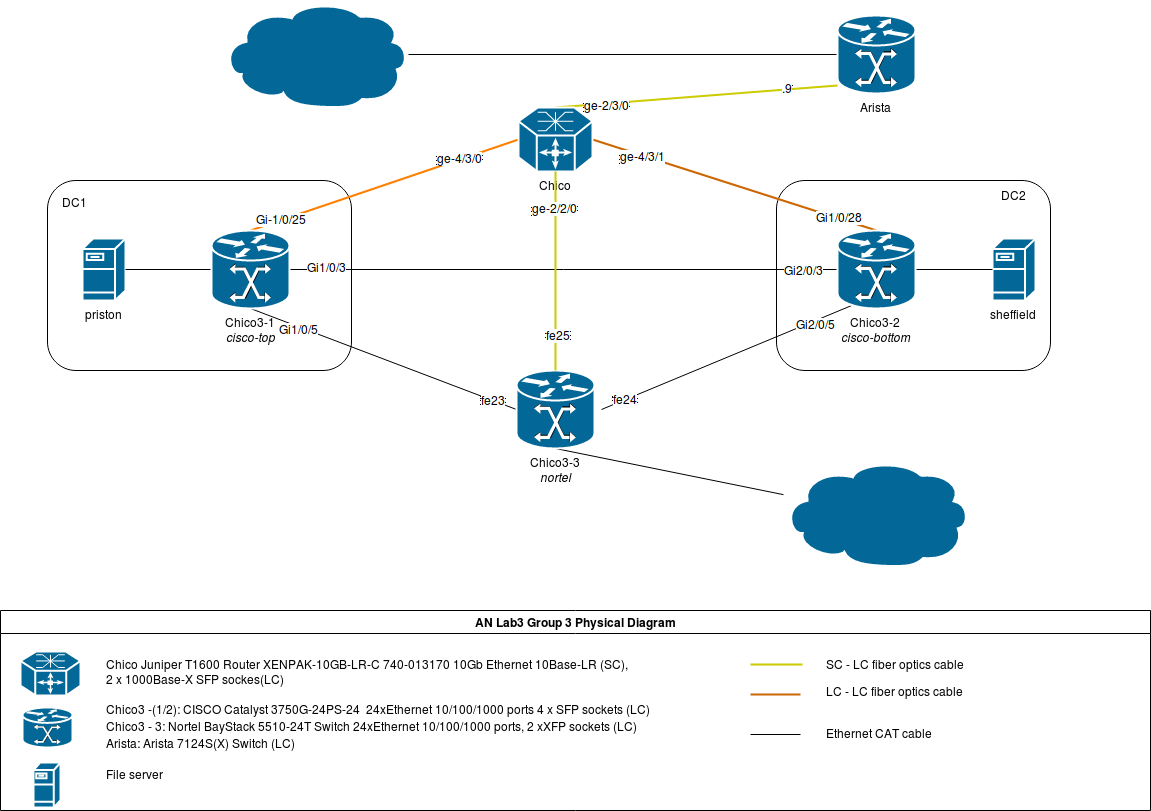
\includegraphics[scale=0.38]{figures/ANLab3Group3PhysicalDia.png}
		\caption{File-sharing network physical design}
	\label{fig:physical-diagram}
\end{figure}

\begin{figure}[H]
	\centering
		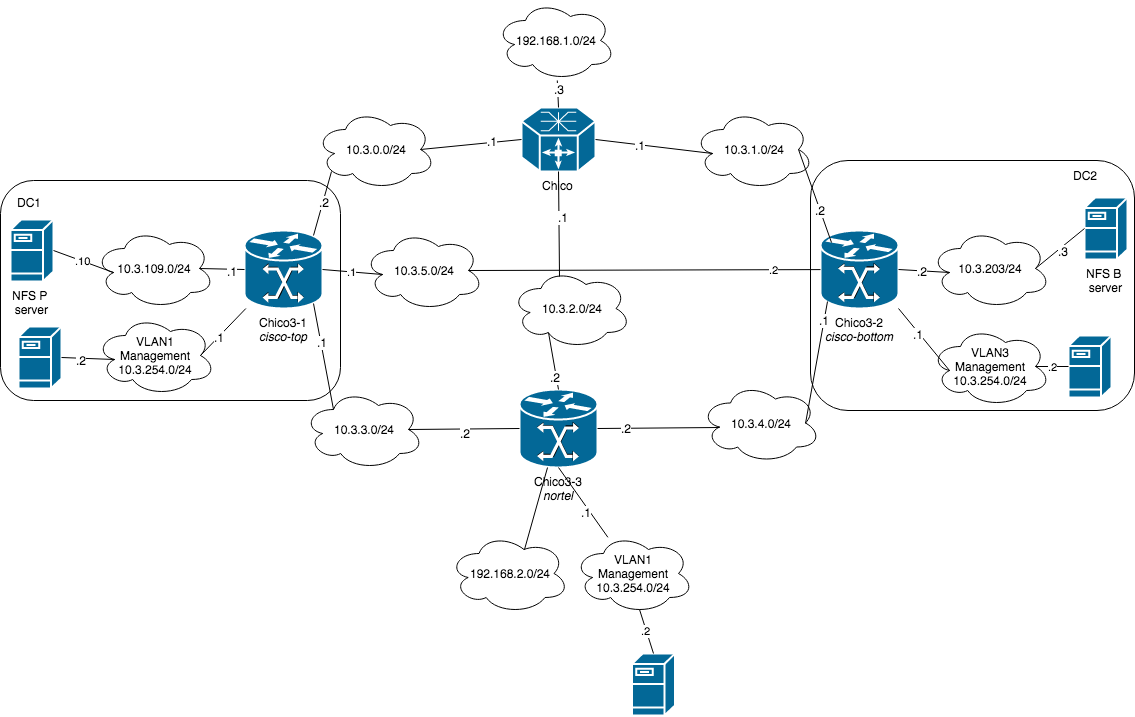
\includegraphics[scale=0.38]{figures/ANLab3Group3LogicalDia.png}
		\caption{File-sharing network logical design}
	\label{fig:logical-diagram}
\end{figure}


The network consists of 4 network devices with routing functionalities, consisting of 2 Cisco Catalyst 3750G-24PS-24 layer 3 switches, 1 Nortel BayStack 5510-24T layer 3 switch and 1 Juniper T1600 router. The connections from the Juniper to the Cisco devices consist of 1 Gbps fiber cables. We have chosen for this redundant set-up to provide multiple paths to access the file-sharing servers. In case one of the routers becomes nonoperational, a different route can be used to reach the NFS servers. In case a router directly connected to NFS drops out, the back-up NFS server can be reached. An attempt to configure the replication process is described in 2.4 Cluster DRBD.
The connection between the Juniper and the Nortel switch is a 10 Gbps link, which is the fastest link in the network. To provide direct access from network DC1 from Chico3-1 to network DC2 at Chico3-2, we have interconnected the Cisco switches with two 1 Gbps copper cables and configured LACP. With LACP the two 1 Gbps links are combined into 1 logical link, providing a bandwidth of 2 Gbps. If one cable breaks, the port channel is still active on 1 Gbps.

The network in \textit{Figure \ref{fig:logical-diagram}} shows two connections between two networks \texttt{192.168.1.0/24} and \texttt{192.168.2.0/24}. Network \texttt{192.168.1.0/24} is used on the OS3 Internet Exchange and is used to peer with group 6, who own 192.168.1.6. Network \texttt{192.168.2.0/24} is used on the direct connection from the Nortel device to the Nortel device of group 6, which provides a redundant network connection to our peer. We have chosen for this to provide a high available storage service for the game server network setup from group 6.

The purpose of the Nortel and Juniper are to provide interconnectivity to peers and the internal network. The two Cisco layer 3 switches are used to provide connectivity to the File-Sharing datacenters. The servers in the topology use the routers to reach eachother and the network outside.

\subsection{The configuration}
The configuration is divided into different parts. First we will describe how we configured the Cisco devices to support SFP modules from a different vendor, then we will describe how we configured LACP. Thirdly, we will describe how we configured the IP-addresses of all interfaces and at last we will describe how we configured the routing protocols and the challenges faced during the configuration.

\subsubsection{Enabling SFP modules from non-cisco vendors}
By default, Cisco does not provide support to SFP-modules manufactured by other vendors. This has to be enabled manually in the configuration. This was done by using the following commands:
\begin{verbatim}
    conf t
    no errdisable detect cause gbic-invalid
    service unsupported-transceiver
\end{verbatim}
After reconnecting the SFP-module, the SFP module works.

\subsubsection{Configuring LACP}
LACP is a protocol used to combine multiple physical links into one logical link \cite{ciscolacp}. This provides a higher bandwidth over a connection and redundancy if one of the links or interfaces break. LACP is configured on interfaces \texttt{G1/0/2} and \texttt{G1/0/3} on Chico3-1 and interfaces \texttt{G2/0/2} and \texttt{G2/0/3} on Chico3-2. The configuration is shown below:

\begin{verbatim}
    conf t
    int G[1 or 2]/0/[switchportnumber]
    no switchport
    channel-group 1 mode active
\end{verbatim}

The port-channel that now appeared in the configuration should get an IP-address. On the side of Chico3-1, the IP-address is configured according to the design shown in \textit{Figure \ref{fig:logical-diagram}}:

\begin{verbatim}
    conf t
    int port-channel 1
    ip addr 10.3.5.1
\end{verbatim}

On the side of Chico3-2, the IP-address is also configured according to the design shown in \textit{Figure \ref{fig:logical-diagram}}:

\begin{verbatim}
    conf t
    int port-channel 1
    ip addr 10.3.5.2
\end{verbatim}

The evidence that the connection over the port-channel works from Chico3-2:
\begin{verbatim}
chico3-2#ping 10.3.5.1

Type escape sequence to abort.
Sending 5, 100-byte ICMP Echos to 10.3.5.1, timeout is 2 seconds:
!!!!!
Success rate is 100 percent (5/5), round-trip min/avg/max = 1/4/9 ms
\end{verbatim}
\\

\subsubsection{Configuring interfaces}
According to the logical network design shown in \textit{Figure \ref{fig:logical-diagram}}, the IP-addresses are configured on the interfaces. On the Juniper, we have configured the IP-addresses as follows:
\begin{verbatim}
    interfaces {
    ge-2/2/0 {
        unit 0 {
            family inet {
                address 10.3.2.1/24;
            }
        }
    }
    ge-2/3/0 {
        unit 0 {
            description to-Zaza;
            family inet {
                address 192.168.1.3/24;
            }
        }
    }
    ge-4/3/0 {
        unit 0 {
            description Internal-1;     
            family inet {
                address 10.3.0.1/24;
            }
        }
    }
    ge-4/3/2 {
        unit 0 {
            family inet {
                address 10.3.1.1/24;
            }
        }
    }
}
\end{verbatim}

On the Cisco devices, we have configured the IP-addresses as follows:
\begin{verbatim}
    conf t
    int G[1/2]/0/[switchportnumber]
    no switchport
    ip addr [ip address] [subnetmask]
\end{verbatim}

On the Nortel devices, we have configured the IP-addresses as follows:
\begin{verbatim}
    brouter port 23 vlan 23 subnet 10.3.3.2/24
    brouter port 24 vlan 224 subnet 10.3.4.2/24
    brouter port 25 vlan 225 subnet 10.3.2.2/24
    brouter port 26 vlan 26 subnet 192.168.2.3/24
\end{verbatim}

\subsubsection{Configuring routing protocols}
In our network we have used of three different routing protocols. BGP is used to communicate with our peers and advertise routes to them. This configuration is described in Task 2. OSPFv2 is used internally in the network to advertise internal and a limited amount of external routes (\texttt{10.6.10.0/24, 10.6.20.0/24 and 10.6.30.0/24}) to internal routers. OSPF is enabled on the Juniper router and the Cisco layer 3 switches. The Nortel switch does not support OSPF without a proper license, therefore we have configured RIP on this device. As the routes advertised through RIP have to be redistributed to OSPF for redundancy, the Cisco devices also have RIPv2 configured. The Juniper router is also directly connected to the Nortel switch, therefore also containing a RIP configuration. In this section we will only cover OSPFv2 and RIPv2 configuration on the Juniper device, Cisco devices and Nortel device. The external routes configured in BGP are covered in Task 2.\\
\\
\textbf{Configuring OSPF}\\
On the Juniper router, OSPF is configured on the interfaces that are connected to the Cisco devices. The interface outside to the peers (\texttt{ge-2/3/0.0}) is set to passive mode. For OSPF, the following features are configured:
\begin{verbatim}
protocols
    ospf {
        export [ bgp-into-ospf rip-into-ospf exportstatic1 direct-into-bgp ];
        area 0.0.0.1 {
            interface ge-4/3/0.0;
            interface ge-4/3/1.0;
            interface ge-2/3/0.0 {
                passive;
            }
        }
    }
\end{verbatim}

The configured area is 0.0.0.1 and the OSPF configuration is accompanied by several policies, which enable the redistribution of BGP traffic into OSPF, RIP traffic into OSPF, Static routes into OSPF and direct routes into OSPF. These policies look as follows:
\begin{verbatim}
    policy-statement bgp-into-ospf {
        term bgpospf {
            from {
                protocol bgp;
                route-filter 10.6.0.0/16 exact;
                route-filter 10.6.10.0/24 exact;
                route-filter 10.6.20.0/24 exact;
                route-filter 10.6.30.0/24 exact;
            }
            then accept;
        }                               
    }
    policy-statement exportstatic1 {
        term exportstatic1 {
            from protocol static;
            then accept;
        }
    }
    policy-statement rip-into-ospf {
        term rip-only {
            from protocol rip;
        }
    }
    policy-statement direct-into-bgp {
        term directbgp {
            from protocol direct;
            then accept;
        }
    }

\end{verbatim}
According to the protocols defined in the policy-statements, the protocols are imported into OSPF. For the policy \texttt{bgp-into-ospf} we have configured that the routes only should be redistributed if the advertised route matches \texttt{10.6.10.0/24}, \texttt{10.6.20.0/24}, \texttt{10.6.30.0/24} or \texttt{10.6.0.0/16}. This is for security, so that other peers on the network can not redistribute routes to their network within our network.

The Cisco routers have a different configuration regarding OSPF:
\begin{verbatim}
Chico3-2:
router ospf 1
 log-adjacency-changes
 redistribute connected
 redistribute rip subnets
 network 10.3.1.0 0.0.0.255 area 0.0.0.1
 network 10.3.5.0 0.0.0.255 area 0.0.0.1
 network 10.3.20.0 0.0.0.255 area 0.0.0.1
 network 10.3.203.0 0.0.0.255 area 0.0.0.1

\end{verbatim}
The directly connected interfaces and RIP classless routes are redistributed into OSPF.
\\
\\
\textbf{Configuring RIP}\\
On the Juniper router, RIP is configured for the interface facing the Nortel router, which is the router that only supports RIP as routing protocol. This was done using the following configuration:
\begin{verbatim}
    rip {
        send broadcast;
        receive version-2;
        group rip-group {               
            export advertise-routes-through-rip;
            neighbor ge-2/2/0.0;
        }
    }

\end{verbatim}

This configuration shows that the RIP version is set to version 2, to support advertising of classless routes. It also shows the policy that direct routes and rip routes should be advertised through RIP. The neighbor interface is \texttt{ge-2/2/0.0}, which is facing the Nortel device.

The Cisco devices also have RIP configured:
\begin{verbatim}
router rip
 version 2
 redistribute connected
 redistribute ospf 1
 network 10.0.0.0
\end{verbatim}

RIP operates on version 2 and redistributes the directly connected connections. It also redistributes the OSPF paths into its own advertisements.

The Nortel device has a different configuration and has to be configured per interface after globally enabling RIP:
\begin{verbatim}
    router rip
    router rip enable
    timers basic holddown 10
    timers basic timeout 20 update 10
    default-metric 8
    network 10.3.2.2
    network 10.3.3.2
    network 10.3.4.2
    network 192.168.2.3
\end{verbatim}

We have changed the values of the timers, such that faster convergence occurs when a route becomes unavailable.

An example of the IP routing table for the Nortel device is shown below:
\begin{verbatim}
    ===============================================================================
                                        Ip Route
===============================================================================
DST             MASK            NEXT            COST    VLAN PORT PROT TYPE PRF
-------------------------------------------------------------------------------
192.168.6.6     255.255.255.255 192.168.2.6     2        26   26    S  IB     5
192.168.2.0     255.255.255.0   192.168.2.3     1        26   ----  C  DB     0
192.168.1.0     255.255.255.0   10.3.2.1        2        225  25    R  IB   100
10.3.203.0      255.255.255.0   10.3.4.1        2        224  24    R  IB   100
10.3.196.0      255.255.255.0   10.3.3.1        2        23   23    R  IB   100
10.3.109.0      255.255.255.0   10.3.3.1        2        23   23    R  IB   100
10.3.5.0        255.255.255.0   10.3.4.1        2        224  24    R  IB   100
10.3.4.0        255.255.255.0   10.3.4.2        1        224  ----  C  DB     0
10.3.3.0        255.255.255.0   10.3.3.2        1        23   ----  C  DB     0
10.3.2.0        255.255.255.0   10.3.2.2        1        225  ----  C  DB     0
10.3.0.0        255.255.255.0   10.3.3.1        2        23   23    R  IB   100
10.3.1.0        255.255.255.0   10.3.4.1        2        224  24    R  IB   100
Total Routes: 12
-------------------------------------------------------------------------------
\end{verbatim}

It only reads RIP and directly connected routes as only RIP is available.

\subsubsection{Testing redundancy}
In this section we describe our test that is performed 5 times to check the time needed for the network to converge after a disruption. We took an average of those 5 times and show examples of the ping and traceroute output. We take server \texttt{sheffield} as source device and first perform a traceroute to 10.3.0.1, which is an interface of the Juniper router:

\begin{verbatim}
rick@sheffield:~$ traceroute 10.3.0.1
traceroute to 10.3.0.1 (10.3.0.1), 30 hops max, 60 byte packets
 1  10.3.203.2 (10.3.203.2)  0.685 ms  0.817 ms  0.982 ms
 2  10.3.5.1 (10.3.5.1)  2.294 ms  2.406 ms  2.559 ms
 3  10.3.0.1 (10.3.0.1)  1.103 ms  1.132 ms  1.108 ms
\end{verbatim}

It shows the route is active through the Etherchannel. First we run a ping and check for disruptions when one of the links that is part of the port channel is disconnected (plugged). We expect LACP automatically recognises the link is unplugged and changes the port count to 1. The results are shown below:
\begin{verbatim}
rick@sheffield:~$ ping -O -D 10.3.0.1 -i 0.2
...
[1520352987.167488] 64 bytes from 10.3.0.1: icmp_seq=86 ttl=62 time=0.518 ms
[1520352987.367395] 64 bytes from 10.3.0.1: icmp_seq=87 ttl=62 time=0.412 ms
[1520352987.567503] 64 bytes from 10.3.0.1: icmp_seq=88 ttl=62 time=0.518 ms
[1520352987.977046] no answer yet for icmp_seq=89
[1520352988.185038] no answer yet for icmp_seq=90
[1520352988.186397] 64 bytes from 10.3.0.1: icmp_seq=91 ttl=62 time=1.27 ms
[1520352988.386128] 64 bytes from 10.3.0.1: icmp_seq=92 ttl=62 time=0.395 ms
[1520352988.586212] 64 bytes from 10.3.0.1: icmp_seq=93 ttl=62 time=0.475 ms
[1520352988.786089] 64 bytes from 10.3.0.1: icmp_seq=94 ttl=62 time=0.361 ms
...
\end{verbatim}

Plugging one of the portchannel cables does show a disruption of 0.2 seconds in the network. Now we'll check the length of the disruption when pulling both portchannel cables:

\begin{verbatim}
    ping -O -D 10.3.0.1 -i 0.2
PING 10.3.0.1 (10.3.0.1) 56(84) bytes of data.
...
[1520352741.227496] 64 bytes from 10.3.0.1: icmp_seq=83 ttl=62 time=0.508 ms
[1520352741.427459] 64 bytes from 10.3.0.1: icmp_seq=84 ttl=62 time=0.466 ms
[1520352741.627384] 64 bytes from 10.3.0.1: icmp_seq=85 ttl=62 time=0.381 ms
[1520352741.827494] 64 bytes from 10.3.0.1: icmp_seq=86 ttl=62 time=0.495 ms
[1520352742.027423] 64 bytes from 10.3.0.1: icmp_seq=87 ttl=62 time=0.434 ms
[1520352742.437050] no answer yet for icmp_seq=88
[1520352742.645041] no answer yet for icmp_seq=89
[1520352742.853053] no answer yet for icmp_seq=90
[1520352743.061035] no answer yet for icmp_seq=91
[1520352743.269040] no answer yet for icmp_seq=92
[1520352743.477048] no answer yet for icmp_seq=93
[1520352743.685045] no answer yet for icmp_seq=94
[1520352743.893054] no answer yet for icmp_seq=95
[1520352744.101043] no answer yet for icmp_seq=96
[1520352744.309034] no answer yet for icmp_seq=97
[1520352744.517087] no answer yet for icmp_seq=98
[1520352744.725045] no answer yet for icmp_seq=99
[1520352744.725701] 64 bytes from 10.3.0.1: icmp_seq=100 ttl=62 time=0.565 ms
[1520352744.925657] 64 bytes from 10.3.0.1: icmp_seq=101 ttl=62 time=0.551 ms
[1520352745.124568] 64 bytes from 10.3.0.1: icmp_seq=102 ttl=62 time=0.465 ms
[1520352745.324649] 64 bytes from 10.3.0.1: icmp_seq=103 ttl=62 time=0.539 ms
[1520352745.524636] 64 bytes from 10.3.0.1: icmp_seq=104 ttl=62 time=0.526 ms
[1520352745.746956] 64 bytes from 10.3.0.1: icmp_seq=105 ttl=62 time=22.8 ms
[1520352745.925785] 64 bytes from 10.3.0.1: icmp_seq=106 ttl=62 time=0.498 ms

...
\end{verbatim}

The downtime is approximately 2 seconds. We now run traceroute again to check which route it is following:

\begin{verbatim}
rick@sheffield:~$ traceroute 10.3.0.1
traceroute to 10.3.0.1 (10.3.0.1), 30 hops max, 60 byte packets
 1  10.3.203.2 (10.3.203.2)  0.778 ms  0.898 ms  1.065 ms
 2  10.3.4.2 (10.3.4.2)  3.168 ms  3.714 ms  4.172 ms
 3  10.3.3.1 (10.3.3.1)  1.856 ms  1.986 ms  2.137 ms
 4  10.3.0.1 (10.3.0.1)  1.201 ms  1.205 ms  1.187 ms
\end{verbatim}

The traffic follows another path, so the redundancy configuration is working and the network is converged within 2 seconds.

\subsubsection{Configure Servers \& Gateway routers}
We already configured the connection between routers through OSPF. The goal of this section is to make the file-servers reach each other through this private network. 

Chico 1:
\begin{verbatim}
    interface GigabitEthernet2/0/11
    no switchport
    ip address 10.3.196.2 255.255.255.0
\end{verbatim}

The ENO2 address set on server Bristol was set to 10.3.196.3/24 with gateway 10.3.196.2. 
ip address 10.3.196.2 255.255.255.0

Chico 2:
\begin{verbatim}
    interface GigabitEthernet2/0/7
    no switchport
    ip address 10.3.203.2 255.255.255.0
\end{verbatim}

The ENO2 address set on server Sheffield was set to 10.3.203.3/24 with gateway 10.3.203.2.

Testing the connection from the gateway:
\begin{verbatim}
chico3-1#ping 10.3.203.2

Type escape sequence to abort.
Sending 5, 100-byte ICMP Echos to 10.3.203.2, timeout is 2 seconds:
!!!!!
Success rate is 100 percent (5/5), round-trip min/avg/max = 1/2/9 ms
chico3-1#ping 10.3.203.3

Type escape sequence to abort.
Sending 5, 100-byte ICMP Echos to 10.3.203.3, timeout is 2 seconds:
!!!!!
Success rate is 100 percent (5/5), round-trip min/avg/max = 1/4/9 ms
\end{verbatim}


\subsection{Network File System}

We have chosen NFS as File-sharing application for this assignment. 

\subsubsection{Overview:}
NFS, or Network File System, is a distributed file system protocol that allows you to mount remote directories on your server. This lets you manage storage space in a different location and write to that space from multiple clients. NFS provides a relatively quick and easy way to access remote systems over a network and works well in situations where the shared resources will be accessed regularly \cite{NFS}. We will set up the NFS between two servers \textbf{Rick-server: 145.100.104.174} client and \textbf{Kotaiba-server: 145.100.104.163} as host. %to-do: fix me

\subsubsection{Configuration:}

\subsubsubsection{Step 1 — Downloading and Installing the Components}

On Host:

\begin{verbatim}
    sudo apt-get update
    sudo apt-get install nfs-kernel-server
\end{verbatim}

On Client:
\begin{verbatim}
    sudo apt-get update
    sudo apt-get install nfs-common
\end{verbatim}


\subsubsubsection{Step 2 — Creating the Share Directories on the Host}

On Host:

\begin{verbatim}
    mkdir /var/nfs/general -p
    chown nobody:nogroup /var/nfs/general
\end{verbatim}

Then I added inside /etc/exports/

\begin{verbatim}
    /var/nfs/general    10.3.203.3(rw,sync,no_subtree_check)
\end{verbatim}

Then restart:
\begin{verbatim}
    systemctl restart nfs-kernel-server
\end{verbatim}

On client:
\begin{verbatim}
    mkdir -p /nfs/general
    mount 10.3.196.3:/var/nfs/general /nfs/general
\end{verbatim}

Check on client:
\begin{verbatim}
root@sheffield:/nfs/general# df -h
Filesystem                        Size  Used Avail Use% Mounted on
udev                              3.8G     0  3.8G   0% /dev
tmpfs                             769M   82M  688M  11% /run
/dev/sda1                         213G  110G   92G  55% /
tmpfs                             3.8G     0  3.8G   0% /dev/shm
tmpfs                             5.0M     0  5.0M   0% /run/lock
tmpfs                             3.8G     0  3.8G   0% /sys/fs/cgroup
10.3.196.3:/var/nfs/general  909G   21G  842G   3% /nfs/general

root@sheffield:/nfs/general# ls
fileCreatedByHost  hellK  RickFanGorp  testNFS

root@sheffield:/nfs/general# cat fileCreatedByHost 
This file was created on Host

\end{verbatim}

NFS access:

\begin{verbatim}
    on Host --> /var/nfs/general
    on Client --> /nfs/general
\end{verbatim}


Now we have working NFS on both servers.


\subsection{Cluster DRBD}
In order to provide a high availability on Application level we used a DRBD cluster. Distributed Replicated Block Device(DRBD) mirrors block devices between multiple hosts. Any block device, such hdd, logical volumes or shares can be mirrored.

In order to privide a High Availability a following parts of environment are used:\\
\textbf{A calais server with IP address 10.3.109.10 is placed on DC1.}\\
\textbf{A sheffield server with IP address 10.3.203.3 is placed in DC2.}

In order to make NFS fail-tolerant, we need to use DRBD. 

\subsubsection{Configuration}
Preparation.
\begin{minted}{bash}
apt-get update
apt-get -y upgrade
\end{minted}

A time synchronisation is required between servers so Network Time Protocol need to be installed on both nodes for accurate time. DRBD heartbeat:
\begin{minted}{bash}
apt-get install -y ntp ntpdate drbd8-utils heartbeat nfs-kernel-server
\end{minted}

Further, hosts file on both nodes needs to be updated by adding following lines:
\begin{minted}{bash}
vim /etc/hosts

10.3.109.10 calais
10.3.203.3 sheffield
\end{minted}

Check disks status:

\begin{minted}{bash}
root@sheffield:/etc# lsblk
NAME                               MAJ:MIN RM   SIZE RO TYPE MOUNTPOINT
sda                                  8:0    0 223.6G  0 disk 
├─sda1                               8:1    0 215.6G  0 part /
├─sda2                               8:2    0     1K  0 part 
└─sda5                               8:5    0     8G  0 part [SWAP]
sdb                                  8:16   0 931.5G  0 disk 
└─sdb1                               8:17   0 119.2G  0 part 
  ├─VolumeGroupXen-Guest--01--swap 252:0    0     1G  0 lvm  
  └─VolumeGroupXen-Guest--01--disk 252:1    0    10G  0 lvm  
loop0                                7:0    0    10G  0 loop 
loop1                                7:1    0     1G  0 loop 

root@calais:~# lsblk
NAME                                MAJ:MIN RM   SIZE RO TYPE  MOUNTPOINT
sda                                   8:0    0 931.5G  0 disk  
├─sda1                                8:1    0 464.5G  0 part  
├─sda2                                8:2    0     1K  0 part  
├─sda5                                8:5    0    16G  0 part  
│ └─cryptswap1                      252:6    0    16G  0 crypt [SWAP]
└─sda6                                8:6    0 451.1G  0 part  /
sdb                                   8:16   0 223.6G  0 disk  
└─sdb1                                8:17   0 119.2G  0 part  
  ├─VolumeGroupXen-Guest--01--swap  252:0    0     1G  0 lvm   
  ├─VolumeGroupXen-Guest--01--disk  252:1    0    10G  0 lvm   
  ├─VolumeGroupXen-Guest--STP--swap 252:2    0     1G  0 lvm   
  ├─VolumeGroupXen-Guest--STP--disk 252:3    0     5G  0 lvm   
  ├─VolumeGroupXen-Guest--LXD--swap 252:4    0     1G  0 lvm   
  └─VolumeGroupXen-Guest--LXD--disk 252:5    0    10G  0 lvm   
root@calais:~# 
\end{minted}

Setting 150M and 10G partitions for both servers:
\begin{minted}
root@calais:~# fdisk /dev/sdb

Welcome to fdisk (util-linux 2.27.1).
Changes will remain in memory only, until you decide to write them.
Be careful before using the write command.


Command (m for help): n
Partition type
   p   primary (1 primary, 0 extended, 3 free)
   e   extended (container for logical partitions)
Select (default p): p
Partition number (2-4, default 2): 2
First sector (250000001-468862127, default 250001408): 
Last sector, +sectors or +size{K,M,G,T,P} (250001408-468862127, default 468862127): +150M       

Created a new partition 2 of type 'Linux' and of size 150 MiB.

Command (m for help): n
Partition type
   p   primary (2 primary, 0 extended, 2 free)
   e   extended (container for logical partitions)
Select (default p): p
Partition number (3,4, default 3): 3
First sector (250000001-468862127, default 250308608): 
Last sector, +sectors or +size{K,M,G,T,P} (250308608-468862127, default 468862127): +10G

Command (m for help): w
The partition table has been altered.
Calling ioctl() to re-read partition table.
Re-reading the partition table failed.: Device or resource busy

The kernel still uses the old table. The new table will be used at the next reboot or after you run partprobe(8) or kpartx(8).


\end{minted}

After reboot. We appended to /etc/drdb.conf (DRBD config) file on both servers with security keeping in mind:
\begin{minted}{bash}
vim /etc/drdb.conf
[..]
common { protocol C; }
resource r0 {
 startup {
    wfc-timeout 30;
    outdated-wfc-timeout 20;
    degr-wfc-timeout 30;
  }
  disk {
    on-io-error detach;
    resync-rate 100M;
  }
  net {
    cram-hmac-alg sha1;
    shared-secret "P@77w0Rd";
  }
  syncer {
    rate 10M;
    al-extents 257;
    verify-alg sha1;
  }
  on calais {
    device /dev/drbd0;
    disk /dev/sdb3;
    address 10.3.109.10:7788;
    meta-disk /dev/sdb2;
  }
  on sheffield {
    device /dev/drbd0;
    disk /dev/sdb3;
    address 10.3.203.3:7788;
    meta-disk /dev/sdb2;
  }
}
\end{minted}


For NFS (/etc/exports) both servers:
\begin{minted}{bash}
/share 10.3.109.10/24(rw,fsid=0,async,no_root_squash,no_subtree_check)   10.3.203.0/24(rw,fsid=0,async,no_root_squash,no_subtree_check)
\end{minted}

Launching drbd both servers:
\begin{minted}{bash}
# modprobe drbd
# drbdadm create-md r0
initializing activity log
NOT initializing bitmap
Writing meta data...
New drbd meta data block successfully created.

# drbdadm up r0
\end{minted}

Sheffield defined as a primary role server so following need to be done:
\begin{minted}{bash}
drbdadm primary --force r0
drbdadm -- --overwrite-data-of-peer primary all
drbdadm -- connect all
\end{minted}

Check connection on both servers:
\begin{minted}{bash}
root@sheffield:~# netstat -tnlp | grep 7788
tcp        0      0 10.3.203.3:7788         0.0.0.0:*               LISTEN      -
\end{minted}

\begin{minted}{bash}
root@calais:~# netstat -tnlp | grep 7788
tcp        0      0 10.3.109.10:7788        0.0.0.0:*               LISTEN      -
\end{minted}

Further on primary server:
\begin{minted}{bash}
mkfs.ext4 /dev/drbd0
mkdir -p /share/nfs/rpc_pipefs/nfs
mount -t ext4 /dev/drbd0 /share
ln -s /share/nfs/ /var/lib/nfs
umount /share
\end{minted}

And secondary:
\begin{minted}{bash}
mkdir -p /share/nfs/rpc_pipefs/nfs
rm -rf /var/lib/nfs/
ln -s /share/nfs/ /var/lib/nfs
\end{minted}

Heartbeat configuration. At this point we came accross a problem where it was clear that hearbeat requires a single public float ip address like 10.3.5.3\cite{BRBD}. However configuration become to complex and by every step provides a error which need to be fixed. It was too complicated to set up in this time frame. We have decided to focus on the networking part.




\section{Task 2: External connections (20 points)}
To establish external connections, we have set up a peering relation with group 6, which is allocated to the Zaza Juniper device. We have agreed to use the external IP: \texttt{192.168.1.3/24} on AS64606.

\subsection{Considerations}
Our network represents a routing network between file-sharing data centers. We do not want other routes than the routes from our peer to be advertised within our network. Therefore we have applied a route-filter on the policy for redistributing BGP traffic into OSPF. The only routes that are allowed to be distributed into OSPF are \texttt{10.6.10.0/24}, \texttt{10.6.20.0/24} and \texttt{10.6.30.0/24} from our external peer group 6. The connectivity to peer group 6 should be redundant, therefore we have two routes to our peer. The external devices are connected to the Nortel router and the Juniper router. The redundancy will work based on the advertised BGP routes and the last resort route configured on the Cisco routers to the Nortel router.

\subsection{Configuration of Juniper}
On the Juniper router we have configured peering and IP-addresses for the interfaces going to the local network. For BGP we have peered with group 6, resulting in the following configuration:
\begin{verbatim}
protocols {
    bgp {
        export [ ospf-into-bgp direct-into-bgp ];
        group external-peers {          
            type external;
            neighbor 192.168.6.6 {
                multihop {
                    ttl 10;
                }
                peer-as 64606;
            }
        }
    }

routing-options {
    static {
        route 192.168.6.6/32 next-hop 192.168.1.6;
    }
    autonomous-system 64603;
}

interfaces{
    ge-2/3/0 {
            unit 0 {
                description to-Zaza;
                family inet {
                    address 192.168.1.3/24;
                }
            }
        }
    }
policy-statement bgp-into-ospf {
        term bgpospf {
            from {
                protocol bgp;
                route-filter 10.6.0.0/16 exact;
                route-filter 10.6.10.0/24 exact;
                route-filter 10.6.20.0/24 exact;
                route-filter 10.6.30.0/24 exact;
            }
            then accept;
        }                               
    }
policy-statement direct-into-bgp {
        term directbgp {
            from protocol direct;
            then accept;
        }
    }
policy-statement ospf-into-bgp {
        term ospf-only {
            from {
                protocol ospf;
                area 0.0.0.1;
            }
            then accept;
        }
    }

\end{verbatim}

The BGP router of Group 6 has the public IP-address \texttt{192.168.6.6} and has the AS-number 64606. The border router of group 6 has IP-address \texttt{192.168.1.6}. Through this border router a peering relation is set up with the BGP router on \texttt{192.168.6.6}. In order to achieve this, \texttt{multihop} must be enabled to allow indirect peering with in our configuration a TTL of 10, so 10 hops are allowed. The policy \texttt{bgp-into-ospf} is used to filter the routes to be advertised into OSPF. The policy \texttt{direct-into-bgp} allows direct connections to be redistributed in BGP and \texttt{ospf-into-bgp} allows OSPF routes to be redistributed in BGP for area 0.0.0.1.

\subsection{Configurations regarding the redundant connection through the Nortel}
We agreed with group 6 that we would provide a redundant connection through the Nortel router. However, the current firmware flashed on the Nortel device does not support BGP. Our firmware was also limited in not being able to use OSPF, so we agreed on setting up some default routes. The default routes that were added to the Nortel device to reach their Nortel device are:
\begin{verbatim}
    192.168.2.0     255.255.255.0   192.168.2.3     1        26   ----  C  DB     0
    0.0.0.0         0.0.0.0         192.168.2.6     2        26   26    S  IB     5
\end{verbatim}

The Cisco switches in the network do not know where to route traffic to if the connection to the Juniper router is down, therefore we have added last resort routes to the Cisco switches to route traffic to the Nortel. The Nortel switch then only forwards the traffic destined for the external network. The last resort route was added using:
\begin{verbatim}
   ip route 0.0.0.0 0.0.0.0 192.168.2.3
\end{verbatim}

\subsection{Testing connectivity}
In order to test the connectivity, we have run a traceroute-request to the IP-address of our peer: \texttt{traceroute 10.6.20.1}.

\begin{verbatim}
chico3-2#traceroute 10.6.20.1
Type escape sequence to abort.
Tracing the route to 10.6.20.1

  1 10.3.5.1 0 msec 0 msec 9 msec
  2 10.3.0.1 0 msec 0 msec 0 msec
  3 192.168.1.6 0 msec 0 msec 0 msec
  4 10.6.1.2 8 msec 0 msec * 

\end{verbatim}

Output of the ping-command:
\begin{verbatim}
chico3-2#ping 10.6.20.1

Type escape sequence to abort.
Sending 5, 100-byte ICMP Echos to 10.6.20.1, timeout is 2 seconds:
!!!!!
Success rate is 100 percent (5/5), round-trip min/avg/max = 1/10/34 ms
\end{verbatim}

The output shows that the connectivity to our peering devices works. We also provide a dump of the BGP routing table on the Juniper:
\begin{verbatim}
    group3@chico:group3> show route 

inet.0: 21 destinations, 30 routes (21 active, 0 holddown, 0 hidden)
+ = Active Route, - = Last Active, * = Both

10.3.0.0/24        *[Direct/0] 4d 00:17:14
                    > via ge-4/3/0.0
                    [RIP/100] 22:02:22, metric 3, tag 0
                    > to 10.3.2.2 via ge-2/2/0.0
10.3.0.1/32        *[Local/0] 4d 01:42:01
                      Local via ge-4/3/0.0
10.3.1.0/24        *[Direct/0] 23:04:44
                    > via ge-4/3/2.0
                    [OSPF/10] 23:04:43, metric 3
                    > to 10.3.0.2 via ge-4/3/0.0
                    [RIP/100] 22:02:22, metric 3, tag 0
                    > to 10.3.2.2 via ge-2/2/0.0
10.3.1.1/32        *[Local/0] 23:06:29
                      Local via ge-4/3/2.0
10.3.2.0/24        *[Direct/0] 22:02:22
                    > via ge-2/2/0.0
10.3.2.1/32        *[Local/0] 4d 01:42:01
                      Local via ge-2/2/0.0
10.3.3.0/24        *[RIP/100] 22:02:22, metric 2, tag 0
                    > to 10.3.2.2 via ge-2/2/0.0
                    [OSPF/150] 22:07:54, metric 20, tag 0
                    > to 10.3.0.2 via ge-4/3/0.0
10.3.4.0/24        *[OSPF/150] 00:00:09, metric 20, tag 0
                    > to 10.3.0.2 via ge-4/3/0.0
10.3.5.0/24        *[OSPF/10] 3d 02:43:16, metric 2
                    > to 10.3.0.2 via ge-4/3/0.0
                    [RIP/100] 22:02:22, metric 3, tag 0
                    > to 10.3.2.2 via ge-2/2/0.0
10.3.109.0/24      *[RIP/100] 02:05:36, metric 3, tag 0
                    > to 10.3.2.2 via ge-2/2/0.0
                    [OSPF/150] 02:05:39, metric 20, tag 0
                    > to 10.3.0.2 via ge-4/3/0.0
10.3.196.0/24      *[OSPF/10] 1d 03:54:43, metric 2
                    > to 10.3.0.2 via ge-4/3/0.0
                    [RIP/100] 22:02:22, metric 3, tag 0
                    > to 10.3.2.2 via ge-2/2/0.0
10.3.203.0/24      *[OSPF/10] 1d 03:42:55, metric 3
                    > to 10.3.0.2 via ge-4/3/0.0
                    [RIP/100] 22:02:22, metric 3, tag 0
                    > to 10.3.2.2 via ge-2/2/0.0
10.6.10.0/24       *[BGP/170] 20:10:17, MED 0, localpref 100, from 192.168.6.6
                      AS path: 64606 I
                    > to 192.168.1.6 via ge-2/3/0.0
10.6.20.0/24       *[BGP/170] 20:10:17, MED 0, localpref 100, from 192.168.6.6
                      AS path: 64606 I
                    > to 192.168.1.6 via ge-2/3/0.0
10.6.30.0/24       *[BGP/170] 20:10:17, MED 0, localpref 100, from 192.168.6.6
                      AS path: 64606 I
                    > to 192.168.1.6 via ge-2/3/0.0
192.168.1.0/24     *[Direct/0] 3d 21:14:37
                    > via ge-2/3/0.0
192.168.1.3/32     *[Local/0] 4d 03:30:29
                      Local via ge-2/3/0.0
192.168.2.0/24     *[RIP/100] 22:02:22, metric 2, tag 0
                    > to 10.3.2.2 via ge-2/2/0.0
                    [OSPF/150] 22:05:25, metric 20, tag 0
                    > to 10.3.0.2 via ge-4/3/0.0
192.168.6.6/32     *[Static/5] 23:00:18
                    > to 192.168.1.6 via ge-2/3/0.0
224.0.0.5/32       *[OSPF/10] 4d 01:24:51, metric 1
                      MultiRecv
224.0.0.9/32       *[RIP/100] 04:15:48, metric 1
                      MultiRecv

\end{verbatim}

The BGP marked routes are the routes advertised by our peers from AS64606.

\section{Task 3: Secure and monitor your network (5 points)}
In order to monitor the network, measures were taken to check the router and switch activity. For this we have set up a Cacti-server, which reads SNMP data from switches and routers. Using this, we can check the throughput of network devices and check whether devices in the network are up or down.\\
\\
Installation and configuration of Cacti:
\begin{verbatim}
    apt install wget patch unzip zip bash-completion
    apt install apache2 libapache2-mod-php7.0 php7.0 php7.0-snmp php7.0-xml \
    php7.0-mbstring php7.0-json php7.0-gd php7.0-gmp php7.0-zip php7.0-ldap php7.0-mcrypt
    apt install build-essential dos2unix dh-autoreconf help2man libssl-dev \
    libmysql++-dev librrds-perl libsnmp-dev
    apt install mariadb-server php7.0-mysql
    
    In MySQL:
    mysql -h localhost -u root -p
    create database cacti;
    grant all on cacti.* to 'cacti_user'@'localhost' identified by 'cacti_pass';
    flush privileges;
    
    For SNMP:
    apt install snmp snmpd snmp-mibs-downloader
    apt install rrdtool
    
    In /etc/snmp/snmpd.conf:
    agentAddress udp:161,udp6:[::1]:161
    rocommunity snmp_string cisco
    
    For Cacti:
    wget https://www.cacti.net/downloads/spine/cacti-spine-latest.tar.gz
    ./configure
    make
    make install
    chown root:root /usr/local/spine/bin/spine
    
    wget https://www.cacti.net/downloads/cacti-latest.tar.gz
    tar xfz cacti-latest.tar.gz
    cp -rf cacti*/* /var/www/html/
    mysql -u cacti_user cacti -p < /var/www/html/cacti.sql
\end{verbatim}

Login details of Cacti:
\begin{verbatim}
    Server: http://145.100.104.174
    Account: admin
    Password: Cisco123!
\end{verbatim}

To allow Cacti to connect to the switches, we have enabled SNMP on all network devices:
\begin{verbatim}
    snmp-server community public RO
\end{verbatim}

Finally we can add manually the devices to the Cacti interface (See Fig. \ref{fig:cacti1}\ref{fig:cacti2}\ref{fig:cacti3}).

\begin{figure}[H]
	\subfigure[Chico3-1 - Cisco]{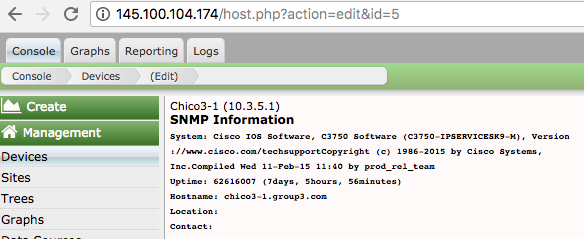
\includegraphics[width=0.4\textwidth]{figures/cacti_chico3-1.png}\label{fig:cacti1}}
\hfill
	\subfigure[Chico3-2 - Cisco]{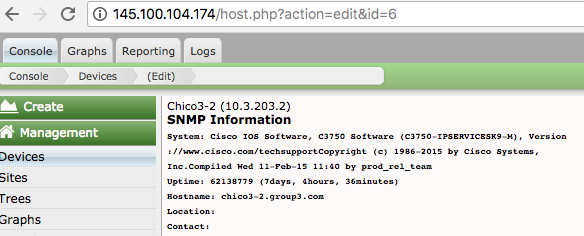
\includegraphics[width=0.4\textwidth]{figures/cacti_chico3-2.png}\label{fig:cacti2}}
\hfill
    \subfigure[Chico3-3 - Nortel]{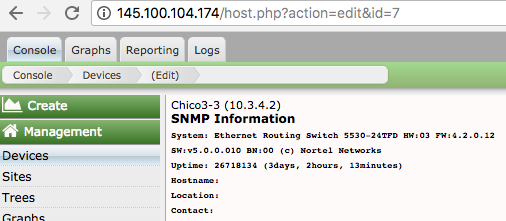
\includegraphics[width=0.4\textwidth]{figures/cacti_chico3-3.png}\label{fig:cacti3}}
\hfill
\end{figure}

From this interface, we can also monitor the port states. Fig. \ref{fig:cacti-ports-monitoring}

\begin{figure}[H]
	\centering
		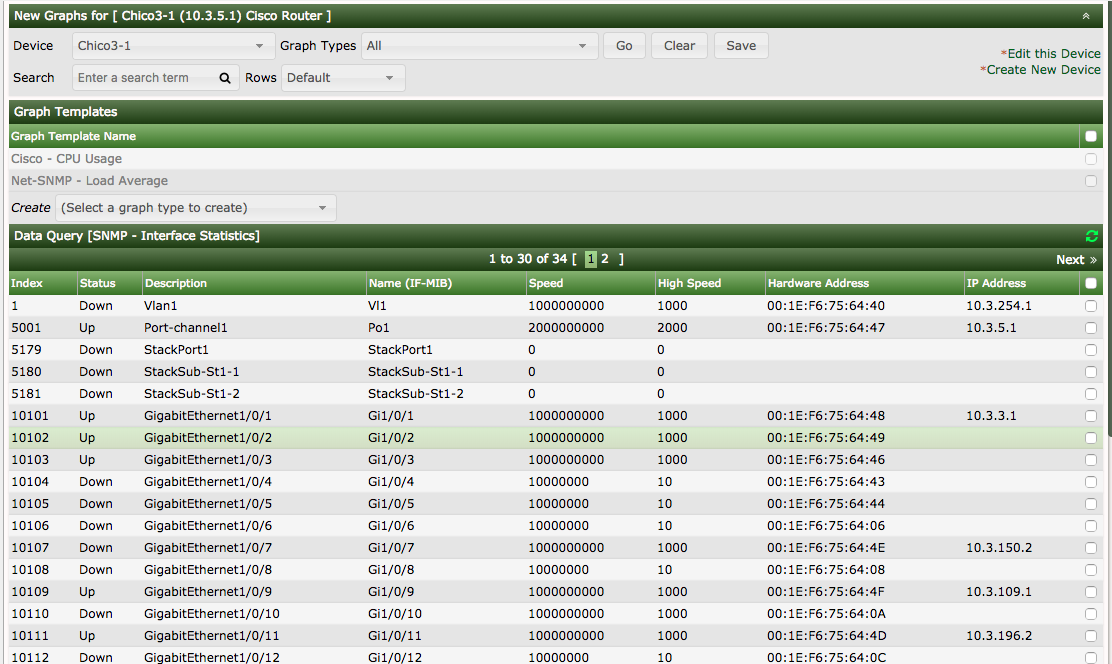
\includegraphics[scale=0.38]{figures/Cacti-ports.png}
		\caption{Cacti port monitoring}
	\label{fig:cacti-ports-monitoring}
\end{figure}

Cacti should be able to plot graphs about the I/O metrics on the switches. However, the back-end server does not seem to be able to build the files to plot. We could not resolve the issue. However, we are sure that the SNMP queries work since the interfaces information are available.

Next to monitoring the network, parts of the network also have to be secured. This can be done by using access lists, but also simple things such as saving the router enable password securely on the Cisco routers. This can be done using \texttt{enable secret 5 [password]}. The password has to be complex and long enough, such that it takes a long time to brute force. As for the access list, on the Cisco devices the access to the datacenter networks can be limited to the internal IP-range \texttt{10.3.0.0/16} and the external peer range \texttt{10.6.0.0/16}. This was configured as follows on the Cisco switches:
\begin{verbatim}
access-list 10 permit 10.3.0.0 0.0.255.255
access-list 10 permit 10.6.0.0 0.0.255.255

interface Port-channel1
 ip access-group 10 in
interface GigabitEthernet2/0/1
 ip access-group 10 in
interface GigabitEthernet2/0/2
 ip access-group 10 in
interface GigabitEthernet2/0/3
 ip access-group 10 in
\end{verbatim}


\section{Discussion}
During this lab we had several limitations in terms of the functionalities provided by the hardware and software. Initially we had a completely different design, where the Cisco devices were interconnected with 4x 1 Gbps links in port channel and the Nortel switch was redunantly connected to the Cisco devices as a switch. Unfortunately, we had problems running compatible Spanning Tree Protocol versions on the Cisco and the Nortel. The Nortel's firmware only supports default STP, where the Cisco devices only supported (R)PVST and MST. Due to these inconsistencies we got switching loops and had to change our network topology to something different (or implement VRRP). We decided to change the topology as group 6 proposed to directly peer our Nortel to their Nortel device, such that there is a redundant connection with our peer.

\newpage

\bibliographystyle{unsrt}
\bibliography{references}


\end{document}
